\documentclass[12pt]{ucalgthes1}
\usepackage[pdftex]{graphicx}
\usepackage[letterpaper,top=1in, bottom= 1in, left= 1in, right= 1in]{geometry}
\usepackage{hyperref}
\usepackage{mathptmx}
\usepackage{listings}
\usepackage{url}
\usepackage{subcaption}
\usepackage{tikz,pgfplots,pgfplotstable}
\usepackage{mathtools}
\usepgfplotslibrary{dateplot}
\usepgfplotslibrary{statistics}
\usepackage{courier}
\usepackage[square,numbers,sectionbib]{natbib}
\usepackage[sectionbib]{chapterbib}
\usepackage[numbib]{tocbibind}
\newcommand{\newblock}{}
\usepackage{eurosym}
\usepackage{multirow}

\title{Title of Thesis (title case, double spaced, no more than 240 characters. No bold font or symbols, except Greek) \\ \bigskip
Thesis Title Second Line }
%
%            Insert the correct information between the {}
%
\author{Student's Full Name}
\thesisyear{year}
\thesis{thesis}    % the word dissertation can be inserted between {}
\newcommand{\thesistitle}{Title of Thesis}
\monthname{month name}
\dept{GRADUATE PROGRAM IN "NAME OF PROGRAM"}
\degree{"FULL NAME OF DEGREE e.g.: DOCTOR OF PHILOSOPHY"}
%
%                    End of supplied information
%
\begin{document}
\makethesistitle
\pagenumbering{roman}     % resets page counter to one
\setcounter{page}{2}
%\chapter*{UNIVERSITY OF CALGARY \\ FACULTY OF GRADUATE STUDIES}
%\thispagestyle{empty}
%The undersigned certify that they have read, and recommend
%to the Faculty of Graduate Studies for acceptance, a \Thesis\ entitled
%``\thesistitle'' submitted by \Author\
%in partial fulfillment of the requirements for the degree of
%\Degree.\\

%
%                 Substitute  List of Examiners
%
%\begin{signing}{Department of Academic Computing}
%\signline
%Chairman, Dr.~John D.~Doe \\
%Department of Academic Computing \\
%Services  \\
%\signline
%Chairman, Dr.~John D.~Doe \\
%Department of Academic Computing \\
%Services  \\
%\signline
%Chairman, Dr.~John D.~Doe \\
%Department of Academic Computing \\
%Services  \\
%\signline
%Chairman, Dr.~John D.~Doe \\
%Department of Academic Computing \\
%Services  \\
%\newsigncolumn         use this command to start a new column if necessary
%\newsigncolumn
%\signline
%Chairman, Dr.~John D.~Doe \\
%Department of Academic Computing \\
%Services  \\
%\signline
%Dr.~Jane Smith \\
%Department of Academic Computing  \\

%\signline
%Dr.~A.~B.~Brown \\
%Department of Academic Computing  \\
%\end{signing}
%
\newpage
\phantomsection
\altchapter{\bf{Abstract}}
Paragraph 1

Paragraph 2

Paragragh 3

This page is required for all graduate theses.  An abstract is a short paragraph explaining the major points and conclusions of your thesis.  For master's theses, the abstract can be no more than 150 words long, while doctoral abstracts can be no longer than 350 words.

\newpage
\phantomsection
\altchapter{\bf{Acknowledgements}}
Paragraph 1

Paragraph 2

Paragraph 3

\begin{singlespace}
\newpage
\phantomsection
\tableofcontents
\pagestyle{plain}
\newpage
\phantomsection
\listoftables
\pagestyle{plain}
\newpage
\phantomsection
\listoffigures
\pagestyle{plain}
\clearpage
\clearpage          % otherwise tables will be numbered wrong
\end{singlespace}
\newpage
\phantomsection
\chapter*{\bf{List of Symbols, Abbreviations and Nomenclature}\hfill} \addcontentsline{toc}{chapter}{List of Symbols}
\listofsymbols
\pagestyle{plain}
\clearpage

\pagenumbering{arabic}
\graphicspath{{controlled_study/}, {case_study/}}
\pgfplotsset{table/search path={controlled_study,case_study}}
\renewcommand\bibname{References}
\usetikzlibrary{backgrounds}
    \label{fig:screenshot_response}
\pgfplotsset{compat=1.5}


\chapter{A Case Study of Web API Evolution}


%\author{\IEEEauthorblockN{S M Sohan, Craig Anslow, Frank Maurer
%\IEEEauthorblockA{Department of Computer Science\\
%University of Calgary,
%Calgary, Alberta T2N 1N4\\ Email: \{smsohan, craig.anslow, frank.maurer\}@ucalgary.ca }
%}}

%\maketitle


\section{Abstract}
When applications are integrated using web APIs, changes on a web API may break the dependent applications. This problem exists because old versions of the APIs may no longer be supported, a lack of adequate documentation to upgrade to a newer version, and insufficient communication of changes. In this paper we conducted a case study of evolving Web APIs to investigate what changes are made between versions and how the changes are documented and communicated to the API users. The findings are a list of recommendations for practitioners and researchers based on API change profiles, versioning, documentation and communication approaches that are observed in practice. This study will help inform developers of evolving Web APIs to make decision about versioning, documentation and communication methods.


%\begin{IEEEkeywords}
%Case Study; RESTful, SOAP, Web API Evolution; WSDL
%\end{IEEEkeywords}

%\IEEEpeerreviewmaketitle

\section{Introduction}

Web APIs are used as a key interconnectivity mechanism to access software services over the Internet. Interconnected applications can provide better service at a lower cost to their users. For example, a business search portal can display the businesses near a user's current location on a map by using the Google Maps API. The actual implementation of Web APIs can follow various protocols, such as SOAP\footnote{http://www.w3.org/TR/soap/} and RESTful\footnote{\url{http://www.ics.uci.edu/~fielding/pubs/dissertation/rest_arch_style.htm}} web services. In this paper, the term Web API is used to describe any protocol unless otherwise specified.

Web APIs connect independently maintained applications. As a result, when a Web API evolves, all the integrated applications using the Web API may not be able to evolve on the same schedule. For example, in the case of the aforementioned business search portal, if the Google Maps API changes, it may also require the portal to change. This introduces unique challenges to the evolution of Web APIs compared because the evolution is out of the control of the API users. For example, API users of a local API can use a copy of an older version, but for evolving Web APIs, API users are forced to upgrade if older versions are no longer supported. Documentation of evolving Web APIs is an important topic for case study because of the unique challenges it presents. Web APIs are defined by their HTTP interface, including both HTTP headers as well as request and response data formats. As a result, for an evolving Web API, its documentation needs to indicate changes in any of these fields, unlike the local APIs, where typically no HTTP specific information is involved.

The primary goal of this research is to investigate the challenges that are currently faced by developers and users of evolving Web APIs so that future research can be performed to address the problems. To this regard, we analyzed existing literature on the topic of Web API evolution. We analyzed the evolution of multiple Web APIs to understand the current industry trends and challenges. The juxtaposition of current industry practices with the literature reveals insights that are otherwise unseen when viewed from a single perspective. We use the differences between the literature and industry practices to identify unresolved research problems.

In this case study, multiple Web APIs representing a variety of application areas are selected, analyzed and compared to gain a broader perspective about current industry practices on Web API versioning, documentation and communication of changes. The result of this analysis is a summary of different approaches to Web API evolution, and a list of recommendations for developers of evolving Web APIs.

The remainder of this paper is organized as follows: the next section is related work on Web API evolution. Then, we discuss the case study of multiple Web API evolution. In the following section, we list our findings, followed by a discussion about the findings. Finally, we conclude with the contributions of this work.

\section{Related Work}

We look at related work in the following areas: Empirical Research on Web API evolution, techniques to evolve Web APIs and, tool support for evolving Web APIs.

\subsection{Empirical Research on Web API evolution} % (fold)
\label{sub:empirical_research}
Several case study papers were published on Web API Evolution. Maleshkova et al. analyzed multiple Web APIs to identify the different approaches related to Web API descriptions, data formats, protocols, reusability, granularity, and authentication \cite{maleshkova}. They found that a lack of a standard format to document Web APIs and manual documentation led to API under-specification causing confusions about how to use the APIs for different use cases. They identified a need for automated approaches.

Fokaefs et al. performed an empirical study on Web API evolution involving multiple SOAP web services, Amazon EC2, FedEx Rate, Bing, Paypal, and Fedex Pack., and provided an evolution profile showing the percentage of changes between two consecutive versions of the Web APIs \cite{fokaefs_2011_empirical}. The same Web APIs were studied by Romano et at., but they provided an alternate evolution profile of the Web APIs. Instead of using percentage of change, they profiled the number of operations, parts and XML file elements from WSDL files for each version of the Web APIs \cite{wsdl_diff_2012}. These change profiles point to the ever changing nature of Web APIs.

Jun et al. performed case studies on the evolution of Web APIs and compared the evolution of Web APIs against local library APIs \cite{li_client_2013}. For studying Web APIs, a selection criteria was provided as follows: Web APIs with large number of clients, covering different application areas, owned by different companies in different countries, and well documented API reference and migration guides. They extracted 16 patterns to describe different types of changes on the Web APIs as follows: add or remove parameter, change type of return value, delete method, rename method, rename parameter, change format of parameter, change format of return value, change XML tag, combine methods, split method, expose data, unsupport request method, change default value of parameter, chance default value of parameter, change upper bound of parameter, restrict access to API. They also presented six challenges specific to Web API evolution that are not found with library APIs such as: transformation between JSON and XML, M to N Mapping, delete method, authorization protocol change, rate limit, and authorization of API access.

Espinha et al. looked at the growing pains with Web API evolution from the perspective of Web API users by conducting interviews \cite{espinha}. The interviewees were selected based on the activity of their open-source projects that used Web APIs. They found that when a Web API evolves, maintaining the integration with a Web API took more effort than integrating it the first time since maintenance is carried out over a longer period of time. This makes the evolution of Web APIs an important subject for a case study.

We distinguish our case study from these case studies as follows: we provide up-to-date information and include a diverse set of Web APIs. Our analysis uses new data sources such as API user forums, and question and answer sites. We focused this study on different approaches to versioning, documentation, and communicating changes as an API evolves.
% subsection empirical_research (end)

\subsection{Techniques to evolve Web APIs} % (fold)
\label{sub:techniques}
Kaminski et al. presented a design technique called ``Chain of Adapters'' to implement evolving Web APIs \cite{kaminski2006design}. Using this approach, the source code of a Web API can evolve from a version to the next by introducing an adapter on the original version to implement any required change for new versions. This technique allows for multiple versions to be deployed concurrently since older versions are left unchanged.

Leskey suggests following a consistent and meaningful naming scheme to identify different versions of APIs \cite{laskey2008considerations}. Such a naming scheme can be used to identify if two versions of an API are compatible. Given the URL scheme, Leskey suggests a self documenting Web API, one that exposes API endpoints to describe the details for each version.

Treiber et al. showed a conceptual model to capture the changes of a Web API \cite{treiber2009analyzing}. A graphical representation to display the evolution of SOAP Web Services is presented by Aversano et al. where the differences between versions are highlighted based on their meta information found in the WSDL files \cite{aversano2005visualizing}.

Some papers focused on automatic migration of Web API clients to newer versions. For example, Wilde proposed a conceptual framework where WSDL can be extended so a client can be compatible with potential Web API changes \cite{wilde2004semantically}. A similar approach is proposed by Fang et al. where a fixed set of new XML nodes are used instead of arbitrary extensions \cite{fang2007version}. Juric et al. proposed a number of versioning related extensions to WSDL that can be applied to version SOAP web services in multiple levels of granularity such as, service level and operation level \cite{Juric20091326}. Zuo et al. developed a formal XML based change specification format to describe the evolution of SOAP Web services \cite{zuo6928972}.

For RESTful Web APIs, Mangler et al. introduced an XML based language called RIDDL \cite{mangler2010origin}. RIDDL allows incremental composition of Web API documentation for different versions by adding a changelog to the documentation of an old version.

VRESCo demonstrates an approach where a router between the Web API client and server is used to automatically route Web API calls to new API versions. The router routes API calls to the desired version based on free form version names such as: latest, stable, and fixed version \cite{leitner2008end}. Meng et al. compared different approaches for evolving Web APIs across multiple criteria: granularity of evolution, terminal of evolution, type of evolution, scalability, and maintainability \cite{6835564}. They identified an aspect oriented approach, where an intermediate tier between a Web API and its clients is used similar to VRESCo, can reduce coupling between the two.

Existing techniques to evolve Web APIs focused on finding different techniques for implementing evolving SOAP based Web APIs that cannot be readily applied to RESTful Web APIs. From our case study, we identified future research opportunities on techniques to solve the problems Web API evolution that are also applicable to RESTful APIs.

\subsection{Tool support for evolving Web APIs} % (fold)
\label{sub:tool_development}


Analyzing the available tool support for evolving Web APIs helped us identify opportunities for future research in this area. WSDarwin introduces a layer of adapters on both the Web API and its client to automatically migrate Web API clients to use a newer version of an API \cite{WSDarwin}. WSDarwin uses WSDL description of the SOAP service to automatically infer the changes between versions and uses preset default values for newly added objects to adapt the client request. VTracker, predecessor of WSDarwin, produces a changelog between versions of WSDL files \cite{fokaefs_2011_empirical}. WSDLDiff extends this by incorporating the semantic meaning of WSDL with an XML Schema Definition into their changelog computation \cite{wsdl_diff_2012}.

To identify if a new version of a Web API has any impact on a specific API client,  Zou et al. show a technique to generate client specific change logs \cite{le2008synchronizing}. A customized per API client change log is generated by filtering the change log based on  recorded API usage data so that only relevant API changes can be communicated effectively to each user.

Existing research on tool support for RESTful Web API evolution is rather limited. hRESTS is an HTML-based specification for describing RESTful Web APIs that can be used by computers to auto-generate client code \cite{4740521}. RESTdesc is another specification for describing RESTful Web API documentation where APIs are described using pre and post conditions \cite{RESTdesc}. However, the input to both hRESTS and RESTDesc require manual effort to produce the desired specification.

In the literature, we found multiple tools exist that rely on WSDL files. WSDL solutions have limited applicability for RESTful Web APIs since WSDL files cannot be used to fully describe RESTful APIs. Based on our case study, we will discuss future research problems on tool development to support the challenges with RESTful Web API evolution.

\section{Case Study}
When companies evolve their Web APIs in practice the new changes can often break applications that rely on these APIs. The aim of this case study is to investigate current industry practices on Web API Evolution to answer the following research questions.

\subsection{Research Questions} % (fold)

\begin{description}
  \item[RQ1] Versioning: How are Web APIs versioned as they evolve?
  \item[RQ2] Documentation: How are Web API changes documented as they evolve?
  \item[RQ3] Communication: How are Web API changes communicated as they evolve?
\end{description}

\subsection{Selection Strategy} % (fold)
\label{sub:selection_strategy}
\begin{table*}[!htbp]
\caption{Case Study - Representative Sample of Web APIs.}
\label{web_api_grid}
\rotatebox{-90}{
  \begin{tabular} {| p{1.5in}| p{2in}| l  | l | l | l | l  | l |}
    \hline
    \multirow{2}{*}{\textbf{Web API}} &
    \multirow{2}{*}{\textbf{URL}} &
    \multicolumn{4}{ c |}{\textbf{Categories}} &
    \textbf{Num of} &
    \multirow{2}{*}{\textbf{Dates}}\\    \cline{3-6}
    & & Industry & Popularity &  Maturity & Code& \textbf{Releases}& \\
    \hline
    Facebook Platform API & \tiny{\url{https://developers.facebook.com/docs/apps/versions}} & Social & High & Est & Closed & 11 & 01/2013-07/2014\\
    \hline
    Twitter REST API & \tiny{\url{https://dev.twitter.com/docs/api}} & Social & High & Est & Closed & 2 & Not Available\\
    \hline
    Wordpress REST API & \tiny{\url{http://wp-api.org/}} & Business & Growing &  New & Open & 8 & 08/2013-06/2014\\
    \hline
    Salesforce \& Chatter REST API & \tiny{\url{https://www.salesforce.com/us/developer/docs/api_rest/}} & Business & Popular & Est & Closed & 4 & 01/2013-08/2014\\
    \hline
    Google Calendar API & \tiny{\url{https://developers.google.com/google-apps/calendar/}} & Business & Popular & Est & Closed & 2 & Not Available\\
    \hline
    Stripe Payment Processor API & \tiny{\url{https://stripe.com/docs/api}} & Business & Growing & New & Closed & 30 &09/2011-10/2014 \\
    \hline
    Github API & \tiny{\url{https://developer.github.com/}} & Productivity & Growing & New & Closed  & 59 &09/2012-10/2014\\
    \hline
    Google Maps API & \tiny{\url{https://developers.google.com/maps/web/}} & Productivity & Popular & Est & Closed & 102 &01/2011-09/2014\\
    \hline
    OpenStreetMap API &\tiny{\url{http://wiki.openstreetmap.org/wiki/API}} & Productivity & Growing & New & Open & 1 & Not Available\\
    \hline
  \end{tabular}
}
\end{table*}



To gain a broad perspective, we selected evolving Web APIs to represent each of the following categories as shown in Table \ref{web_api_grid}.

\textbf{Industry} - APIs representing different domains: social, business, and productivity.

\textbf{Popularity} - APIs with different number of users.

\textbf{Maturity} - Newer vs. established Web APIs.

\textbf{Source code} - Open source vs. closed source.


\subsection{Research Method - Qualitative Analysis} % (fold)
\label{sub:research_method}

The APIs in this case study are proprietary and open-source evolving Web APIs. For each API, we collected publicly available data from the following sources: API home page, formal API reference, and user forums and question-answer sites. A homepage provides a general introduction to the Web API. The formal API reference described the different elements of the API. The user forums and question-answer sites are used to communicate news and collect feedback about the Web APIs, for example StackOverflow.com.

The first author of this paper read the the API homepages and followed relevant hyperlinks to find answers to RQ1. A summary of the strategies were presented to the co-authors, which was used to categorize Web API versioning strategies into groups. Web API homepages contain changelogs and links to API references which were used to find answers to RQ2.

We used codes to annotate the API changelogs to identify the different types of API changes. The coding scheme started with a set of codes based on the codes from Jun et al. \cite{li_client_2013}. New codes  emerged from our analysis as the existing codes did not describe an API change scenario. An overview of the used codes is provided in Table \ref{coding_scheme}. The codes were applied to the different API elements as described through the following example Web API description:

``A Web API to post a comment on a photo.''

\textbf{Endpoint} - URLs to access the the API.
\textbf{Resource} - An input or output object. For example, comment, photo, etc.
\textbf{Method} - An API operation on a resource. e.g. post a comment.
\textbf{Field} - An attribute of the resource. e.g. timestamps of a comment.
\textbf{FieldValue} - Possible value for a field. For example: a timestamp value of January 1, 2015.
\textbf{Error} - Error cases. e.g. not found error.
\textbf{Authentication} - Authentication methods. e.g. HTTP Basic authentication.


\begin{table*}[!htbp]
\caption{List of Codes}
\label{coding_scheme}
\begin{tabular}{|p{0.3\linewidth}|p{0.6\linewidth}|}
\hline
\textbf{Category} & \textbf{Description}\\
\hline
Add$<$APIElements$>$ & New API elements introduced: Adds a new resource, field, field value, endpoint or method\\
\hline
Remove$<$APIElements$>$ & API elements completely removed: Removes a resource, field, field value, endpoint or method\\
\hline
Change$<$APIElements$>$ & Existing API element is replaced by another: Replaces or renames a resource, field, field value, endpoint or method\\
\hline
ErrorConditionChange & Changes the possible error conditions: New, changed or removed error response \\
\hline
ChangeFieldDataType & Changes the data type of a field: Single item to an array or vice versa, number to strings or vice versa, required to optional or vice versa\\
\hline
BehaviorChange & Changes the outcome or fixes bug: Uses new formula for computing API return values\\
\hline
ChangeAuthentication & Changes how API clients are authenticated: New, changed or deprecated API authentication methods\\
\hline
ChangeAuthorization & Changes who can access which API elements: Add, remove or modify permissions of API user\\
\hline
\end{tabular}
\end{table*}

These codes were applied to the text from the Web API homepages and API changelogs for multiple versions to produce a change profile. The first and second authors of this paper arrived at the same conclusion when they independently applied the  codes on 18 snippets of changelogs randomly sampled from the studied Web APIs. The coding process was manual since the data comprises of unstructured text that are not suitable for automated tagging. Here is an example of a change log from WordPress API with the codes:

\small
``Add post meta endpoints \textbf{(AddEndpoint)}.
Creating, reading, updating and deleting \textbf{(AddMethod * 4)}
post meta \textbf{(AddResource)} is now possible by
using \url{the/posts/<id>/meta} endpoints.''
\normalsize

We analyzed the API user forums and newsboards to find answers to RQ3. Messages in these sources were filtered to focus on the evolution of Web APIs. These data sources provided the perspectives of both the developers and users of Web APIs. To find evolution related messages, based on trial search runs, full text search features on the forums were used to search for these keywords: version, release, migration, breaking, deprecate, change.


\section{Findings} % (fold)
\label{sec:findings}

In this section we present our findings for RQ1-3.

\subsection{RQ1 Versioning} % (fold)
\label{sub:versioning}


\subsubsection{Patterns of Changes}

Based on our coding scheme, we identified the following new change patterns to describe changes between versions of Web APIs in addition to the 16 patterns described by Jun et al. \cite{li_client_2013} as follows:

\textbf{Move API elements} - We found 114 occurrences of element moves, where API elements are moved under new hierarchy or renamed. For example, Stripe API moved two objects under a new API element as found in the following change log from version 2013-08-13:

\small
\begin{quotation}
``Remove fee and fee\_details properties on charge and transfer objects. Instead, fee information is now stored on the corresponding balance transaction.
''\end{quotation}
\normalsize

\textbf{Rename API elements} - We found that 31 API elements were renamed for consistency. The following example from the Facebook API shows a rename \footnote{\url{https://developers.facebook.com/docs/apps/migrations/ads-api-changes-2014-07-02}}:

\small
\begin{quotation}
``Facebook will be renaming the adgroup\_status value ADGROUP\_PAUSED TO PAUSED to be consistent with the rest of the object's APIs.
''\end{quotation}
\normalsize

\textbf{Behavior change} - We have found 247 examples where Web APIs changed the resultant data while keeping the API interfaces intact. These are commonly triggered by bug fixes. For example, Wordpress REST API 1.1 changed as follows \footnote{\url{http://make.wordpress.org/core/2014/06/23/json-rest-api-version-1-1/}}:

\small
\begin{quotation}
``Correct password-protected post handling.
Password-protected posts could previously be exposed to all users, however
could also have broken behavior with excerpts. Password-protected posts are
now hidden to unauthenticated users..
''\end{quotation}
\normalsize

Another example that demonstrates a behavior change can be found from the 2013-10-29 version of Stripe API \footnote{\url{https://stripe.com/docs/upgrades\#2014-01-31}}:

\small
\begin{quotation}
``When we apply a \$Y coupon to a \$X dollar invoice, we are no longer applying the remainder of the coupon to the account balance if Y $>$ X. Applications of coupons to \$0 invoices will no longer count as a redemption of the coupon.''
\end{quotation}
\normalsize

\textbf{Post condition change} - In the studied Web APIs we found examples where the immediate result of an API call remained unchanged but new post conditions are imposed requiring additional work for the API users. The following change on Facebook platform API illustrates this \footnote{\url{https://developers.facebook.com/docs/apps/migrations/payments-disputes-realtime-updates-required-2014-05-13}}:

\small
\begin{quotation}
``Starting May 13th, 2014, developers that accept payments will be required to subscribe to and honor Realtime Updates to ensure order fulfillment and appropriate handling of disputes from all payers. If you do not subscribe to and honor these updates, Facebook reserves the right, under our Developer Payment Terms to withhold payouts and/or stop your app from accepting payments.
''\end{quotation}
\normalsize

\textbf{HTTP header change} - Web APIs also change the custom HTTP headers that are used as meta data. For example, the following shows a change when the WordPress Web API introduced two new headers to describe the pagination status of an API call \footnote{\url{http://make.wordpress.org/core/2013/09/12/json-rest-api-version-0-5/}}:

\small
\begin{quotation}
``Send X-WP-Total and X-WP-TotalPages headers for information on post/pagination counts''
\end{quotation}
\normalsize

Similarly, the Github API changed their custom headers about pagination in the following example \footnote{\url{https://developer.github.com/v3/versions/}}:

\small
\begin{quotation}
``No longer using the X-Next or X-Last headers. Pagination info is returned in the Link header instead.''
\end{quotation}
\normalsize

\textbf{Error condition change} - Web APIs change the error conditions that may require the users to adapt their integration. For example, in Salesforce API Version 29 the error codes were changed \footnote{\url{https://na1.salesforce.com/help/pdfs/en/salesforce_winter14_release_notes.pdf\#rn_186_api_objects}}:

\small
\begin{quotation}
``...different ExceptionCode and StatusCode values are now returned for some error conditions
when saving user records. We strongly recommend that you test your code and modify it accordingly if your clients rely on specific ExceptionCode and StatusCode values being returned...
''\end{quotation}
\normalsize

These extended list of change patterns need to be addressed by future work on finding techniques and developing tool support for evolving Web APIs.


\subsubsection{Version Identifiers}

We analyzed different approaches to identify the versions of Web APIs to understand if the version identifiers can be used to infer information about their evolution. We can categorize the Web APIs into these groups:
\textbf{Numbered identifiers} - Contiguous integers are used to identify new versions by Salesforce and GitHub Web APIs. Such naming scheme clearly communicates the sequence between versions but cannot be used to infer compatibility between versions.

\textbf{Timestamped identifiers} - Stripe Web API uses date as a version identifier. While timestamped versions provide the time frame of a version, they do not provide any compatibility information between versions.

\textbf{Identifiers with major and minor version numbers} - Most of the Web APIs studied use major and minor version numbers to identify a version. Facebook, Twitter, WordPress, Google Calendar, Google Maps and OpenStreetMap follow this approach. However, an explanation of the major and minor version numbers aren't provided and cannot be used to infer compatibility information.

Also, web APIs often evolve with breaking changes without issuing a new version identifier. For example, Facebook, Google Calendar and GitHub APIs often receive breaking changes without using a new version identifier.




\begin{figure*}[!hbtp]
  \begin{subfigure}[b]{\textwidth}
    \def\dataSourceFileName{facebookx.dat}
    \begin{tikzpicture}[show background rectangle,tight background]
      \begin{axis}[
          ybar stacked,
          bar width=5pt,
          date coordinates in=x,
          xticklabel = \year-\month,
          xtick = {2013-01-09, 2013-04-01, 2013-07-01, 2013-10-01, 2014-01-01, 2014-04-01, 2014-08-01, 2014-07-02},
          xlabel style={font=\small},
          ylabel style={font=\small},
          ylabel={No. of Changes},
          xticklabel style= {rotate=90,anchor=near xticklabel,font=\tiny},
          enlarge x limits=false,
          height=0.20\textheight,
          width=\textwidth,
          legend style={legend pos=north west,font=\tiny, legend columns=4},
          legend to name=legend
        ]
        \addplot[fill=green] table[x=Date, y=AddAPIElements]{plotdata/\dataSourceFileName}
\closedcycle;
\addplot[fill=red] table[x=Date, y=RemoveAPIElements]{plotdata/\dataSourceFileName}
\closedcycle;
\addplot[fill=orange] table[x=Date, y=ChangeAPIElements]{plotdata/\dataSourceFileName}
\closedcycle;
\addplot[fill=gray] table[x=Date, y=ChangeFieldDataType]{plotdata/\dataSourceFileName}
\closedcycle;
\addplot[fill=violet] table[x=Date, y=ErrorConditionChange]{plotdata/\dataSourceFileName}
\closedcycle;
\addplot[fill=yellow] table[x=Date, y=ChangeAuthentication]{plotdata/\dataSourceFileName}
\closedcycle;
\addplot[fill=magenta] table[x=Date, y=BehaviorChange]{plotdata/\dataSourceFileName}
\closedcycle;
\addplot[fill=blue] table[x=Date, y=ChangeAuthorization]{plotdata/\dataSourceFileName}
\closedcycle;

\legend{AddAPIElements, RemoveAPIElements, ChangeAPIElements,
  ChangeFieldDataType, ErrorConditionChange,
  ChangeAuthentication, BehaviorChange, ChangeAuthorization}

      \end{axis}
    \end{tikzpicture}
    \caption{Facebook API Changes (11 Releases)}
    \label{fig:facebook-chart}
  \end{subfigure}

  \begin{subfigure}[b]{\textwidth}
    \def\dataSourceFileName{stripe.dat}
    \begin{tikzpicture}[show background rectangle,tight background]
      \begin{axis}[
          date coordinates in=x,
          ybar stacked,
          bar width=5pt,
          xticklabel = \year-\month,
          xtick = {2011-09-15, 2012-01-01, 2013-01-01, 2014-01-01, 2014-10-01},
    %xlabel={Timeline},
          xlabel style={font=\small},
          ylabel style={font=\small},
          ylabel={No. of Changes},
          xticklabel style= {rotate=90,anchor=near xticklabel,font=\tiny},
          enlarge x limits=false,
          height=0.20\textheight,
          width=\textwidth,
          legend to name=legend
        ]
        \addplot[fill=green] table[x=Date, y=AddAPIElements]{plotdata/\dataSourceFileName}
\closedcycle;
\addplot[fill=red] table[x=Date, y=RemoveAPIElements]{plotdata/\dataSourceFileName}
\closedcycle;
\addplot[fill=orange] table[x=Date, y=ChangeAPIElements]{plotdata/\dataSourceFileName}
\closedcycle;
\addplot[fill=gray] table[x=Date, y=ChangeFieldDataType]{plotdata/\dataSourceFileName}
\closedcycle;
\addplot[fill=violet] table[x=Date, y=ErrorConditionChange]{plotdata/\dataSourceFileName}
\closedcycle;
\addplot[fill=yellow] table[x=Date, y=ChangeAuthentication]{plotdata/\dataSourceFileName}
\closedcycle;
\addplot[fill=magenta] table[x=Date, y=BehaviorChange]{plotdata/\dataSourceFileName}
\closedcycle;
\addplot[fill=blue] table[x=Date, y=ChangeAuthorization]{plotdata/\dataSourceFileName}
\closedcycle;

\legend{AddAPIElements, RemoveAPIElements, ChangeAPIElements,
  ChangeFieldDataType, ErrorConditionChange,
  ChangeAuthentication, BehaviorChange, ChangeAuthorization}

      \end{axis}
    \end{tikzpicture}
    \caption{Stripe API Changes (30 Releases)}
    \label{fig:stripe-chart}
  \end{subfigure}

  \begin{subfigure}[b]{\textwidth}
    \def\dataSourceFileName{wordpress.dat}
    \begin{tikzpicture}[show background rectangle,tight background]
      \begin{axis}[
    %title=WordPress REST API Changes (8 Releases),
          date coordinates in=x,
          ybar stacked,
          bar width=5pt,
          xticklabel = \year-\month,
          xtick = {2013-08-07, 2013-11-01, 2014-03-01, 2014-06-26},
    %xlabel={Timeline},
          xlabel style={font=\small},
          ylabel style={font=\small},
          ylabel={No. of Changes},
          xticklabel style= {rotate=90,anchor=near xticklabel,font=\tiny},
          enlarge x limits=false,
          height=0.20\textheight,
          width=\textwidth,
          legend to name=legend
        ]
        \addplot[fill=green] table[x=Date, y=AddAPIElements]{plotdata/\dataSourceFileName}
\closedcycle;
\addplot[fill=red] table[x=Date, y=RemoveAPIElements]{plotdata/\dataSourceFileName}
\closedcycle;
\addplot[fill=orange] table[x=Date, y=ChangeAPIElements]{plotdata/\dataSourceFileName}
\closedcycle;
\addplot[fill=gray] table[x=Date, y=ChangeFieldDataType]{plotdata/\dataSourceFileName}
\closedcycle;
\addplot[fill=violet] table[x=Date, y=ErrorConditionChange]{plotdata/\dataSourceFileName}
\closedcycle;
\addplot[fill=yellow] table[x=Date, y=ChangeAuthentication]{plotdata/\dataSourceFileName}
\closedcycle;
\addplot[fill=magenta] table[x=Date, y=BehaviorChange]{plotdata/\dataSourceFileName}
\closedcycle;
\addplot[fill=blue] table[x=Date, y=ChangeAuthorization]{plotdata/\dataSourceFileName}
\closedcycle;

\legend{AddAPIElements, RemoveAPIElements, ChangeAPIElements,
  ChangeFieldDataType, ErrorConditionChange,
  ChangeAuthentication, BehaviorChange, ChangeAuthorization}

      \end{axis}
    \end{tikzpicture}
    \caption{WordPress REST API Changes (8 Releases)}
    \label{fig:wordpress-chart}
  \end{subfigure}
  \begin{subfigure}[b]{\textwidth}
    \def\dataSourceFileName{github.dat}
    \begin{tikzpicture}[show background rectangle,tight background]
      \begin{axis}[
    %title=GitHub API Changes (59 Releases),
          date coordinates in=x,
          ybar stacked,
          bar width=5pt,
          xticklabel = \year-\month,
          xtick = {2012-09-05, 2012-12-01, 2013-03-01, 2013-06-01, 2013-09-01, 2013-12-01, 2014-03-01, 2014-10-06},
    %xlabel={Timeline},
          xlabel style={font=\small},
          ylabel style={font=\small},
          ylabel={No. of Changes},
          xticklabel style= {rotate=90,anchor=near xticklabel,font=\tiny},
          enlarge x limits=false,
          height=0.20\textheight,
          width=\textwidth,
          legend to name=legend
        ]
        \addplot[fill=green] table[x=Date, y=AddAPIElements]{plotdata/\dataSourceFileName}
\closedcycle;
\addplot[fill=red] table[x=Date, y=RemoveAPIElements]{plotdata/\dataSourceFileName}
\closedcycle;
\addplot[fill=orange] table[x=Date, y=ChangeAPIElements]{plotdata/\dataSourceFileName}
\closedcycle;
\addplot[fill=gray] table[x=Date, y=ChangeFieldDataType]{plotdata/\dataSourceFileName}
\closedcycle;
\addplot[fill=violet] table[x=Date, y=ErrorConditionChange]{plotdata/\dataSourceFileName}
\closedcycle;
\addplot[fill=yellow] table[x=Date, y=ChangeAuthentication]{plotdata/\dataSourceFileName}
\closedcycle;
\addplot[fill=magenta] table[x=Date, y=BehaviorChange]{plotdata/\dataSourceFileName}
\closedcycle;
\addplot[fill=blue] table[x=Date, y=ChangeAuthorization]{plotdata/\dataSourceFileName}
\closedcycle;

\legend{AddAPIElements, RemoveAPIElements, ChangeAPIElements,
  ChangeFieldDataType, ErrorConditionChange,
  ChangeAuthentication, BehaviorChange, ChangeAuthorization}

      \end{axis}
    \end{tikzpicture}
    \caption{GitHub API Changes (59 Releases)}
    \label{fig:github-chart}
  \end{subfigure}



\end{figure*}
\begin{figure*}[!h]\ContinuedFloat


  \begin{subfigure}[b]{\textwidth}
    \def\dataSourceFileName{gmap.dat}
    \begin{tikzpicture}[show background rectangle,tight background]
      \begin{axis}[
    %title=Google Maps Web API (102 Releases),
          date coordinates in=x,
          ybar stacked,
          bar width=5pt,
          xticklabel = \year-\month,
          xtick = {2011-01-06, 2011-07-01, 2012-01-01, 2012-07-01, 2013-01-01, 2013-07-01, 2014-01-01, 2014-07-01, 2014-09-18},
    %xlabel={Timeline},
          xlabel style={font=\small},
          ylabel style={font=\small},
          ylabel={No. of Changes},
          xticklabel style= {rotate=90,anchor=near xticklabel,font=\tiny},
          enlarge x limits=false,
          height=0.20\textheight,
          width=\textwidth,
          legend to name=legend
        ]
        \addplot[fill=green] table[x=Date, y=AddAPIElements]{plotdata/\dataSourceFileName}
\closedcycle;
\addplot[fill=red] table[x=Date, y=RemoveAPIElements]{plotdata/\dataSourceFileName}
\closedcycle;
\addplot[fill=orange] table[x=Date, y=ChangeAPIElements]{plotdata/\dataSourceFileName}
\closedcycle;
\addplot[fill=gray] table[x=Date, y=ChangeFieldDataType]{plotdata/\dataSourceFileName}
\closedcycle;
\addplot[fill=violet] table[x=Date, y=ErrorConditionChange]{plotdata/\dataSourceFileName}
\closedcycle;
\addplot[fill=yellow] table[x=Date, y=ChangeAuthentication]{plotdata/\dataSourceFileName}
\closedcycle;
\addplot[fill=magenta] table[x=Date, y=BehaviorChange]{plotdata/\dataSourceFileName}
\closedcycle;
\addplot[fill=blue] table[x=Date, y=ChangeAuthorization]{plotdata/\dataSourceFileName}
\closedcycle;

\legend{AddAPIElements, RemoveAPIElements, ChangeAPIElements,
  ChangeFieldDataType, ErrorConditionChange,
  ChangeAuthentication, BehaviorChange, ChangeAuthorization}

      \end{axis}
    \end{tikzpicture}
    \caption{Google Maps Web API (102 Releases)}
    \label{fig:gmaps-chart}
  \end{subfigure}


  \begin{subfigure}[b]{\textwidth}
    \def\dataSourceName{Salesforce Force.com and Chatter REST}
    \def\dataSourceFileName{salesforce.dat}
    \begin{tikzpicture}[show background rectangle,tight background]
      \begin{axis}[
    %title=Salesforce REST API (4 Releases),
          date coordinates in=x,
          ybar stacked,
          bar width=5pt,
          xticklabel = \year-\month,
          xtick = {2013-10-04, 2014-01-01, 2014-04-01, 2014-07-01, 2014-10-18},
    %label={Timeline},
          xlabel style={font=\small},
          ylabel style={font=\small},
          ylabel={No. of Changes},
          xticklabel style= {rotate=90,anchor=near xticklabel,font=\tiny},
          enlarge x limits=false,
          height=0.20\textheight,
          width=\textwidth,
          legend to name=legend
        ]
        \addplot[fill=green] table[x=Date, y=AddAPIElements]{plotdata/\dataSourceFileName}
\closedcycle;
\addplot[fill=red] table[x=Date, y=RemoveAPIElements]{plotdata/\dataSourceFileName}
\closedcycle;
\addplot[fill=orange] table[x=Date, y=ChangeAPIElements]{plotdata/\dataSourceFileName}
\closedcycle;
\addplot[fill=gray] table[x=Date, y=ChangeFieldDataType]{plotdata/\dataSourceFileName}
\closedcycle;
\addplot[fill=violet] table[x=Date, y=ErrorConditionChange]{plotdata/\dataSourceFileName}
\closedcycle;
\addplot[fill=yellow] table[x=Date, y=ChangeAuthentication]{plotdata/\dataSourceFileName}
\closedcycle;
\addplot[fill=magenta] table[x=Date, y=BehaviorChange]{plotdata/\dataSourceFileName}
\closedcycle;
\addplot[fill=blue] table[x=Date, y=ChangeAuthorization]{plotdata/\dataSourceFileName}
\closedcycle;

\legend{AddAPIElements, RemoveAPIElements, ChangeAPIElements,
  ChangeFieldDataType, ErrorConditionChange,
  ChangeAuthentication, BehaviorChange, ChangeAuthorization}

      \end{axis}
    \end{tikzpicture}
    \caption{Salesforce REST API (4 Releases)}
    \label{fig:salesforce-chart}
  \end{subfigure}

%% Add the legend here
  \begin{center}
    \begin{subfigure}[b]{10cm}
      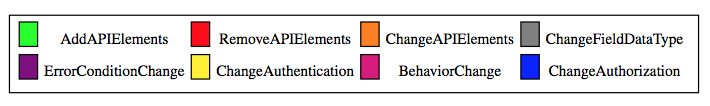
\includegraphics[keepaspectratio, width=10cm]{legend.png}
      \caption{Legend}
    \end{subfigure}
  \end{center}
  \caption{Case Study - Change Profiles for the Web APIs.}
  \label{fig:proflie}
\end{figure*}

\subsubsection{Upgrade Mode} % (fold)

From our case studies, we found the Web APIs followed several different approaches to versioning.

\textbf{Single Version} - Web APIs that force the API clients to migrate either because only one version is available or deprecated older versions will be removed. These include Facebook REST API (90 days), Twitter REST API (no specific time frame), Github API (no specific time frame), OpenStreetMap API (no specific time frame), Google Calendar (6 months), Google Maps (no specific time frame).

\textbf{Multiple Versions} - Multiple versions of the Web API are supported for longer duration. These include Wordpress REST API, Salesforce API, Stripe API.

Both of these categories, single and multiple available versions, have their advantages and disadvantages. Forcing API clients to use a single stable version makes it easy to maintain the Web APIs at the expense of scheduling flexibility for API users. These APIs keep a deprecated version for a limited period of time to provide a buffer time for the API users. For example, Google Calendar API is supporting its deprecated version for 6 months.

Maintaining multiple versions of the Web APIs provide more scheduling flexibility to the API clients but requires more effort from the API publisher. As a result, not all the older versions are maintained. When API clients lag far behind the latest version, migrating to the latest version becomes harder. For example, here is an excerpt of a comment from a Stripe Web API client developer \footnote{\url{https://groups.google.com/a/lists.stripe.com/forum/\#!searchin/api-discuss/version/api-discuss/x8TM-yHnhYQ/y9JJKytSiUAJ}}:

\small
``...I just learned that we're about 14 versions behind and would like to work on upgrading but there are lots of breaking changes...''
\normalsize

While both the forced and on demand modes are found in practice, future work needs to be carried out to compare and contrast the benefits of these modes in greater detail.




\subsubsection{Change Profiles}
The Web APIs evolve at different frequencies as well as the actual change that takes place during their evolution varies from one API to another. Fig. \ref{fig:proflie} shows an aggregated view of the count of different categories of changes observed for different Web APIs based on the aforementioned coding scheme.


The APIs here show very different change trajectories. Facebook API shows an alternating pattern of smaller and larger number of changes between subsequent versions, and each release consists of multiple categories of changes. On the other hand, Stripe and GitHub API changes are more frequent, but on the majority of the releases only include a single category of change. WordPress REST API releases contain multiple categories of changes, but shows only a single API element removal for the studied period. GoogleMaps API changes are also very frequent, dominated by AddAPIElement and BehaviorChange categories in a way that once new API elements are introduced, the subsequent releases primarily focus on bug fixes. The GoogleMaps API shows signs of stability with time. The Salesforce API changelog shows a different picture. Unlike the other APIs studied, Salesforce API evolves quarterly and involves a larger number of API elements with each release. We observed most Web API releases broke backward compatibility as shown by the presence of colors in addition to the green areas on the charts. We consider API changes to be backward compatible when changes are limited to only AddAPIElements category.

Google Calendar API, not shown in a chart, changed the format of all API request and response data from a custom XML to JSON in a single release, effectively forcing all its users to upgrade with a deprecation policy of one year. A plot for the Twitter and OpenStreetMap APIs could not be produced since changelogs for these APIs were no longer available.

These change profiles have little similarity, implying the fact that a common solution to solve their evolution related challenges may not work. Future research on Web API evolution needs to consider these variation of change profiles to find effective solutions for the case in hand.

\subsubsection{Implementation} % (fold)
\label{ssub:implementation}

In our case studies, we included two open-source Web APIs, WordPress and OpenStreetMap, because it gave us access to  their source code to study how versioning is actually implemented. Wordpress REST API is developed as a plugin for Wordpress. As a result, a new version of the Web API is released with a new version of the plugin and it all API clients are affected when a new version is deployed. The source code for OpenStreetMap.org Web API shows the use of configuration files for API Versioning. We found its implementation only allows for a single API version.

To summarize the change profiles, version identifiers and implementation of evolving Web API versions, we observed little convergence and a lack of any common scheme that was followed by the studied Web APIs.

\subsection{RQ2 Documentation} % (fold)
\label{sub:documentation}
Web API documentation is used by API users as the primary source of information for system integration. We analyzed the API reference documentation to understand the contents and the presentation style of their documentation. The documentation is commonly comprised of the following:

\textbf{Web API access information} - Web API documentation includes information about the URL where the API can be reached. The studied APIs used one of the URL, HTTP headers, or a user interface to identify specific API versions.

\textbf{Authentication} - Web API documentation includes information about authentication for their API clients. This is also used to implement client specific rules, such as rate limits and time zones.

\textbf{API Interface definition} - The interface definition is a major part of the Web API documentation where each API element is described with a general overview  and related business rules.

\textbf{Example usage} - Examples that describe different use cases of the Web APIs are also commonly found in the documentation. The examples contain the data and HTTP headers for sample requests and the corresponding API responses.

Some of the studied Web APIs also provide live web browser based API explorers, where API users can make API calls without needing to write any code. However, the studied Web APIs that offered Live API Explorer only did so for the latest API versions.

Web API documentation needs to include additional information compared to local APIs since HTTP is used for communication. As an API evolves lack of documentation for older API versions causes difficulties with the upgrade process as found in the following comment from a Stripe API user\footnote{\url{https://groups.google.com/a/lists.stripe.com/forum/\#!searchin/api-discuss/version/api-discuss/li4PyVcweiw/NT9SFTtF-vQJ}}

\small
\begin{quotation}
 ``Does the full API documentation only reflect the current version of the
  API?  Is there a way to access the API docs for outdated versions? ...That would be very helpful. When you are trying to upgrade from one version to another it's impossible to know the implementation differences. We are currently about 4 API versions behind and are stuck behind a version that causes a significant amount of work on our end to support. I'd like to be able to upgrade incrementally through each version.''
\end{quotation}
\normalsize

We also investigated how the API documentation is generated. We found that, Web API documents are manually generated and updated, unlike the documentation for local APIs which are are typically auto-generated. For WordPress and OpenStreetMap, this is apparent from their source code, as we found the use of manually edited wiki and Markdown files to generate the documentation\footnote{\url{http://en.wikipedia.org/wiki/Markdown}}.

In our case studies, we found one example of self-documenting Web API as discussed by Laskey \cite{laskey2008considerations}. The Salesforce Web API has API endpoints that describe all available versions of the API that can be used to programmatically determine the changes between versions.

To summarize, we found that Web API documents are manually generated and widely vary in terms of both their contents and presentation formats.

\subsection{RQ3 Communication} % (fold)
\label{sub:communication}

Communicating updates and changelogs is an important activity for evolving Web APIs. The communication channels used by the studied Web APIs is categorized as follows:


  \textbf{API home page} - Web APIs announce the API changes in their home pages. In practice, the announcements include partial change log with the key changes that are made in a release. These announcements are unstructured text and do not follow any standard format even for the same API.

  \textbf{API response} - Some Web APIs use custom HTTP headers to indicate when a call is made to a deprecated version. For example, Wordpress REST API sends the X-WP-DeprecatedFunction header in response to API calls made to deprecated endpoints.

  \textbf{Email} - Facebook sends customized email alerts to its API clients based on their usage of the API, similar to the idea as presented by Zou et al. \cite{le2008synchronizing}. API calls are recorded to determine if a change has an impact on users. The granularity of the change tracking often results into false-positives, as found in this comment by a Facebook API user \footnote{\url{http://stackoverflow.com/questions/16270446/updating-app-for-breaking-change-non-threaded-comments}}:

\small
\begin{quotation}
...I have received the same notification for one of my apps. My app definitely does not read or create comments on Facebook posts or objects ... Thus Facebook's message is not relevant to every app they send it to.
The change should only affect apps which read or publish comments.
\end{quotation}
\normalsize

  \textbf{Newsfeed} - To keep up-to-date with API changes, the Web API clients are requested to subscribe to newsfeed, typically delivered via mailing lists and Twitter feeds. User feedback is also collected on these platforms. For example, at the time of writing this paper there were 13,239 questions tagged against google-maps-api-3\footnote{\url{https://stackoverflow.com/questions/tagged/google-maps-api-313.239}}.


To summarize, we found both formal and informal channels are used to communicate Web API changes. Most messages are primarily driven by manually edited unstructured text.
% subsection communication (end)

\section{Discussion} % (fold)
\label{sec:discussion}
Our case study findings such as a lack of standard approaches to deal with Web API versioning, documentation and change communication confirms the findings from previous case studies. In addition to the Web API change patterns identified by previous case studies, we have identified six new change patterns: 1) move API elements, 2) rename API elements, 3) behavior change, 4) post condition change, 5) HTTP header change, and 6) error condition change. When creating API changelog and developing related tool support, these new change patterns can be used to communicate the changes using a shared vocabulary. In addition to these new change patterns, from our case study we have compiled a list of recommendations and identified new research problems related to RQ1-3 as discussed in the following paragraphs.

\textbf{RQ1 Versioning} - From our case study, we found that when a new version is released for a Web API, the version identifiers provide little information about backward compatibility and the impact of the new version on existing API users. As a result, the API users are left to follow the free-form newsfeeds to understand the impact for each new API version. To improve this situation, for practitioners, we recommend using Semantic Versioning. Semantic Versioning is a naming technique for versioning software so that it is possible to infer if two versions are backward compatible simply by interpreting the version identifiers\footnote{\url{http://semver.org/}}. Future research can be carried out to automatically generate a Semantic Versioning identifier based on the compatibility between versions.

Our change profiles show that Web APIs often evolve as fast as several times a month and forces API clients to upgrade. Also, releases often combine both bug fixes and other breaking changes, forcing the API users to adapt even though they only need the fixes.  For practitioners, we recommend that bug fixes and breaking changes be released under separate versions to provide more flexibility to the API clients. Future research needs to focus on finding strategies for evolving Web APIs so that bug fixes and other changes can be easily delivered in separate versions and multiple versions can be made available at the same time.

\textbf{RQ2 Documentation} - We observed a that largely manual process is used for generating API documentation for most RESTful APIs. Manually generating and maintaining such documentation is expensive and error-prone. From our analysis, we showed that even when Web APIs are  versioned, documentation for older versions is not always available, and the difference between two versions of a Web API cannot be easily derived from their manually edited API references. We also found that the changelogs and API references are two disconnected documents even though a user needs to read both documents while upgrading. For practitioners, we recommend releasing Web API documentation for each available version that is cross-linked with the changelog. Future research on tool development can be aimed to support automated, version-aware documentation needs of evolving Web APIs.

Live Web API explorers are used by API users to try the APIs with little effort. However, there is a lack of reusable approach to create Live Web API explorers and bespoke implementation of the live API explorers are expensive since they need additional software development. We have seen only two of the nine studied APIs to provide a live API explorer. Moreover, we found that live Web API explorers are only offered for latest versions. Future research can focus on the implementation of a reusable, version-aware live Web API explorer for evolving Web APIs.

Self documenting Web APIs can be used to automatically determine compatibility between two versions of a Web API. We found Salesforce REST API to be the only example from our case studies that implemented self documenting Web APIs. For practitioners, we recommend providing self-documenting Web APIs. We also identify this as an opportunity for future research so that reusable tool support can be provided to create self-documenting Web APIS.

\textbf{RQ3 Communication} - For communicating API changes, we found a number of different channels that are used in practice. These channels need to be compared so that the effective channels can be used for communicating between the API developers and users.

In the change profiles we found the APIs change frequently and this requires manual effort to understand the impact of a change on a specific API user. This can be simplified by alerting users about an API change with a customized changelog. We also found that API related discussions are carried out external to the API documentation sites. API users need to search multiple disconnected information sources when API related questions arise. For practitioners, we recommend publishing a customized changelog for their Web APIs and providing discussion forums with API documentation. Previous research showed a solution based on WSDL files \cite{le2008synchronizing}. Future research is needed to solve this problem for RESTful Web APIs.

The open source Web APIs (Wordpress and OpenStreetMap) had limited documentation and change log information compared to the proprietary Web APIs. This presents an opportunity for researchers and industry practitioners to create reusable open source versioning and documentation tools for evolving Web APIs.

\textbf{Limitations} - We recognize the number of Web APIs studied to be a threat to the construct validity. Although our selection involves a diverse set of Web APIs, the findings may not be generalized for all evolving Web APIs. Our selection criteria included different industry domains, API sizes, popularity and maturity levels to minimize selection bias. The selected APIs represent only publicly available evolving Web APIs because only publicly available data is used for the case study. Future work need to be carried out to compare the applicability of our findings and related implications on privately maintained evolving Web APIs. To mitigate the interpretation bias of the coding scheme, the first two authors of this paper independently annotated randomly selected snippets of change logs from different Web APIs and reached the same conclusion indicating the replicability of the given coding scheme.

Given the state of practice we found a wide variety of ways to evolve Web APIs in terms of versioning, documentation and communication of changes and no consistent way to deal with the changes. This indicates an immature area where cost-effective solutions that are acceptable for both API developers and users are still missing - as discussed. Further research needs to be carried out to validate the usefulness of the aforementioned recommendations and solve the new research problems as identified by this case study.

\section{Conclusion}
Web API evolution poses challenges since a change may break applications that are developed by different teams and organizations. We presented a case study of Web API evolution focusing on the challenges involved with versioning, documentation and communication of API changes. Recommendations for practitioners from our analysis include the use of semantic versioning, separate releases for bug fixes and new features, auto generated API documentation cross-linked with changelogs and providing live API explorers. A list of open research problems are discussed related to Web API evolution that we want to solve in our future work.

\bibliographystyle{IEEEtran}
\bibliography{IEEEabrv,case_study/references}


%\documentclass[conference]{IEEEtran}


%\ifCLASSINFOpdf
  %\usepackage{listings}
  %\usepackage[pdftex]{graphicx}
  %\usepackage{url}
  %\usepackage{subcaption}
  %\usepackage{tikz,pgfplots,pgfplotstable}
  %\usepackage{mathtools}
  %\usepgfplotslibrary{statistics}
  %\usepackage{courier}
%\else
%\fi

%\makeatletter
%%%%%%%%%%%%%%%%%%%%%%%%%%%%%%% User specified LaTeX commands.
%\def\ps@IEEEtitlepagestyle{%
  %\def\@oddfoot{\mycopyrightnotice}%
  %\def\@evenfoot{}%
%}
%\def\mycopyrightnotice{%
  %{\footnotesize 978-1-5386-0443-4/17/\$31.00 ©2017 IEEE\hfill}% <--- Change here
  %\gdef\mycopyrightnotice{}% just in case
%}
%\begin{document}
%\title{A Study of the Effectiveness of Usage Examples in REST API Documentation}
\chapter{A Study of the Effectiveness of Usage Examples in REST API Documentation}


 %\author{\IEEEauthorblockN{S M Sohan, Frank Maurer\IEEEauthorrefmark{1}}
 %\IEEEauthorblockA{\IEEEauthorrefmark{1}
 %Dept. of Computer Science\\
 %University of Calgary\\
 %Canada\\
 %\{smsohan, frank.maurer\}@ucalgary.ca}
 %\and
 %\IEEEauthorblockN{Craig Anslow}
 %\IEEEauthorblockA{School of Eng. and Computer Science\\
 %Victoria University of Wellington\\
 %New Zealand\\
 %craig@ecs.vuw.ac.nz}
 %\and
 %\IEEEauthorblockN{Martin P. Robillard}
 %\IEEEauthorblockA{
 %School of Computer Science\\
 %McGill University\\
 %Canada\\
 %martin@cs.mcgill.ca}
 %}

%\maketitle

\section{Abstract}
Generating and maintaining REST API documentation with usage examples can be a time consuming and expensive process for evolving APIs. Most REST API documentation tools focus on automating the documentation of the API objects, but require manual effort for capturing usage examples. Consequently, REST API developers need to know the cost vs. benefit of providing usage examples in the documentation to prioritize the documentation efforts. To this end, we have performed a controlled study with 26 experienced software engineers to understand problems that REST API client developers face while using an API without usage examples. We found that REST API client developers face productivity problems with using correct data types, data formats, required HTTP headers and request body when documentation lacks usage examples. By following the REST API documentation suggestions from this paper, REST API developers can reduce the errors, improve success rate and satisfaction of API client developers.



%\begin{IEEEkeywords}
%API; REST; Documentation; Usage Examples; Empirical Study; Controlled Study; Productivity;

%\end{IEEEkeywords}

%\IEEEpeerreviewmaketitle


\section{Introduction}
REST APIs are used as the predominant application integration mechanism over the Internet. Generating and maintaining REST API documentation with usage examples can be an expensive process because most API documentation tools do not support effective usage examples. Researchers have emphasized API documentation as a key factor that impacts API usability both positively and negatively. To improve API documentation, researchers have recommended incorporating usage examples in the API documentation.

In a resource constrained environment, it is important to understand the value of usage examples on REST API usability to allocate sufficient attention and efforts towards incorporating examples in the API documentation. While it is expected that examples help API client developers, API developers need to know what to include in the examples and why.

The documentation of REST APIs has distinctive features compared to the documentation of local APIs such as Java libraries. For example, local API documentation commonly comprises the description of classes and interfaces with their methods. In contrast, REST API documentation needs to include information about HTTP headers, request and response body and the data representation formats such as JSON, XML. The existing research on API usability areas have primarily focused on local APIs. In our work we have focused on understanding the impact of usage examples within the realm of the distinctive REST API features.

We designed and performed a controlled study with experienced software engineers to understand how REST API client developers are affected while using an API documentation that describes the API elements but lacks usage examples. Participants were divided into two groups and given the same set of API tasks to complete. One group was given the official WordPress REST API documentation and another group was given an enhanced version of the documentation where three usage examples were added. Using a novel technique, we collected 539 API calls made by the participants. We analyzed the data and observed recurring obstacles faced by the participants while performing the API tasks using the official documentation that lacks usage examples. Our contributions on this paper are as follows:

\begin{itemize}
  \item We provide a list of obstacles that REST API client developers face while performing API tasks using documentation that lacks usage examples.
  \item We provide a list of recommendations for REST developers to be used as a guideline to incorporate usage examples in API documentation.
  \item We provide empirical evidence that usage examples in REST API documentation help API client developers perform API tasks with higher developer satisfaction, less time, and better success rate.
\end{itemize}

The remainder of this paper is organized as follows: In Section \ref{sec:goal} we present our research question. In Section \ref{sec:method} we discuss our methodology in terms of the study requirements, the selected API of the study and the participant selection, the study setup, data collection and analysis methods. In Section \ref{sec:results} we discuss the results of our analysis. We discuss the threats to validity and provide a summary of the related work in Sections \ref{sec:threat} and  \ref{sec:related_work} respectively.

\section{Research Question}
\label{sec:goal}
This research is aimed at answering the following question:

\begin{itemize}
  \item \textbf{RQ}. What obstacles do API client developers face when using a REST API documentation that lacks usage examples?
\end{itemize}

\section{Methodology} % (fold)
\label{sec:method}

To answer the aforementioned research question, the study has the following requirements:

\begin{itemize}
  \item \textbf{R1. Representative API.} We had to choose an existing REST API that is currently used by API client developers. Selecting a mature REST API for this study reduces the possibility that the obstacles we observe in the study are the results of insignificant accidental problems symptomatic of an immature technology. We selected a familiar domain so that participants are able to relate to the API features without requiring upfront training. In addition to selecting the API, we had to select tasks that are related to the core features provided by the API to represent a common usage area of the API.
  \item \textbf{R2. Open source.} To be able to understand the impact of usage examples, we needed to select an open-source API where we can add new examples to the documentation for performing this study.
  \item \textbf{R3. Time bound.} We applied a maximum time constraint for each participant to measure the rate of success within a limited time frame. As a result, the study needs to be setup such that participants are able to focus on performing the tasks minimizing any overhead.
  \item \textbf{R4. Participant Selection.} Developers with prior experience on REST APIs need to be recruited as study participants to perform the study within a limited amount of time and in a realistic setup. Furthermore, to reduce a learning bias, only participants with no prior experince of using the WordPress REST API V2 are accepted for this study.
\end{itemize}


\subsection{Study API} % (fold)

We selected the WordPress REST API V2 for this study. WordPress is a blog-like open-source (R2) framework used by over 409 million people to visit 23.6 billion pages each month \footnote{\url{https://wordpress.com/activity/}}. The API allows programmatic access to list, create, update, and delete WordPress data such as blog posts, comments, users, images, and tags.

The WordPress REST API V2 has been published and maintained since May 2015. Before January 2017, the WordPress REST API V2 was distributed as a plug-in where WordPress users could optionally install the API component. The following statistics are for the plug-in installation numbers between May 2015 and October 2016:\footnote{\url{https://wordpress.org/plugins/rest-api/stats/}}

\begin{itemize}
  \item Total installations: $ \approx 248K$ installs of the plug-in.
  \item Average daily installations: $ \approx 500$.
\end{itemize}

Starting January 2017, the WordPress REST API V2 is no longer required to be installed as a separate plug-in since it is bundled with WordPress installation. According to the code repository, there are a total of 99 and 46 contributors that had at least one commit to the code repository of the API and its documentation, respectively. These properties satisfy R1 AND R2, our requirements for using a representative API. By selecting an open-source project we are able to access the source-code to inspect the implementation and documentation technique of the WordPress REST API. The API implements a self-documenting feature where API developers expose API endpoints over HTTP OPTIONS verb to explain the API elements. To implement this feature, the API developers describe the API elements in the code. For example:

\lstset{basicstyle=\ttfamily\footnotesize,breaklines=true}
\begin{lstlisting}[language=php,showspaces=false,showstringspaces=false,numbers=left,xleftmargin=2em,caption={Example of self-documenting API Code in PHP},label=wordpress_code]
public function get_item_schema() {
  $schema = array(
    '$schema'    => 'http://json-schema.org/draft-04/schema#',
    'title'      => $this->post_type,
    'type'       => 'object',
    /*
     * Base properties for every Post.
     */
    'properties' => array(
        'date'            => array(
            'description' => __( "The date the object was published, in the site's timezone." ),
            'type'        => 'string',
            'format'      => 'date-time',
            'context'     => array( 'view', 'edit', 'embed' ),
        ),...
\end{lstlisting}

On Listing \ref{wordpress_code}, line 4 specifies that this is a schema definition for the API element \lstinline{Post} \footnote{\url{https://github.com/WP-API/WP-API}}. On Line 10, it defines \lstinline{date}, one of the properties of \lstinline{Post}, followed by a human readable description and type information. On line 14, the context of this property is mentioned as \lstinline{view, edit, embed}, meaning that this property will be returned when the \lstinline{Post} object is returned, embedded, or can be used as an input for editing.

The WordPress team leverages this self-documenting feature to generate and publish the official API documentation as an HTML website. Fig. \ref{fig:schema} shows a screenshot of the published documentation for the \lstinline{date} attribute of the \lstinline{Post} API element.\footnote{\url{http://v2.wp-api.org/reference/posts/}}

\begin{figure}
  \begin{center}
    \fbox{\includegraphics[width=\linewidth,keepaspectratio]{schema.png}}
  \end{center}
  \caption{Screenshot of Documentation for Post/date}
  \label{fig:schema}
\end{figure}

In addition to the auto-generated documentation of the the schema and API actions, contributors add custom content to provide prosaic overviews and usage examples.



\subsection{Study Design} % (fold)
\subsubsection{Tasks} % (fold)

The participants are requested to perform a total of six tasks using the API including one practice task. All of the tasks are related to a single API element, \lstinline{Post}\footnote{A Post identifies a blog post within WordPress}. The tasks get progressively more difficult, and all but the last task can be performed independently of each other. Participants are requested to limit the total time on the study to a maximum of one hour (R3). Participants are encouraged to proceed to the next task when they are either satisfied with their answer or feel stuck and unable to make progress.

To use a REST API, the API client developers need to work with the following four inputs over HTTP:

\begin{itemize}
  \item I1. Request method
  \item I2. Request URL
  \item I3. Request headers
  \item I4. Request body
\end{itemize}

To verify the response of an API call, the API client developers can use HTTP response headers and/or HTTP response body. To perform the tasks, the participants are required to use one or more of the inputs I1-4. In the following paragraphs, we describe each task with its description and the study observation goals against the aforementioned API input and output information. For each of the tasks, the participants are required to use the same WordPress REST API and one of the two variants of accompanying documentation.

\textbf{T1: List all posts task}. We asked the participants to use the WordPress REST API to get a list of the blog posts from a given WordPress site. This is the practice task, and the inputs to answer this task are pre-filled for the participants. It allows the participants to understand the tools used for this study as well as get familiarity with the Post API. The answer for this task makes use of I1 and I2.

\textbf{T2: Filter posts by author task.} The participants are asked to use the API to filter the list of posts obtained in T1 by an author given the author's user name. To answer this correctly, the participants are required to first make an API call to get the numeric ID of the author given the string based user name. Then, the ID needs to be used on the \lstinline{Post} API to filter posts by the author. This task allows us to understand the impact of usage examples on API client developers when multiple API calls need to be made to perform a task using the API. Inputs I1-2 are required to complete this task successfully.

\textbf{T3: Exclude posts by IDs task.} We ask the participants to use the API to get a list of all posts excluding posts with IDs 1 and 4. Participants need to use the inputs I1-2, and use a desired format on I2 to pass an array of IDs as a parameter. This task allows us to understand how API client developers identify the format for using an array within the URL with respect to the usage examples in the API documentation.

\textbf{T4: Find total posts task.} This task requires the participants to use the API to find a total number of posts. Participants need to use the inputs I1-2 and inspect the HTTP response headers to successfully complete this task. This task allows us to understand how API client developer productivity is affected with respect to missing examples about HTTP response headers in the API documentation.

\textbf{T5: Publish post task.} We ask the participants to use the API to publish a blog post with a specific title, content, and a published date. To successfully complete this task, the participants are required to use all four input types and inspect both the HTTP response header and the response body. Additionally, the participants are required to use a specific date format that the API accepts as a valid format for date specification. Answers to this task allows us to study API client developer productivity with respect to the usage examples lacking details about the inputs I3-4.

\textbf{T6: Update post task.} We ask the participants to use the API to update a blog \lstinline{Post} that they published in T5 with a new \lstinline{excerpt}. Similar to T5, this task requires the use of inputs I1-4, but with different values for the inputs. This task allows us to understand API client developer productivity on inter-dependent tasks with respect to usage examples.

To summarize, the tasks allow us to understand how REST API client developers approach API tasks of different complexity levels involving various input types and available output information with respect to the usage examples in the API documentation.

\subsubsection{Participant Selection} % (fold)

To satisfy the requirement of developers with REST API experience (R4), we used the following criteria for recruiting the study participants:

\begin{itemize}
  \item Currently working as a software engineer.
  \item At least 1 year of industry experience as a developer.
  \item At least 1 year of industry experience with REST APIs.
  \item No prior experience with WordPress REST API.
\end{itemize}


\begin{figure*}[t]
\begin{center}
\fbox{\includegraphics[width=\linewidth,keepaspectratio]{api_explorer.png}}
\end{center}
\caption{Screenshot of the Custom-built Web-based REST API Explorer Used by Study Participants}
\label{fig:api_explorer}
\end{figure*}


We recruited a total of 26 participants from sixteen different companies and six different countries (Canada, USA, Germany, Ireland, Brazil, and,
Bangladesh) through online announcements posted on Twitter, Facebook, and software developer focused mailing lists. Table \ref{table:participants} shows a summary of the experience level of the participants in each group.

\begin{table}[!tbh]
  \centering
  \caption{Participant Profile}
  \label{table:participants}

  \begin{tabular}{|p{1.5in} p{1in} p{1.5in} p{1.5in}|}

\hline
& & \textbf{Group 1} & \textbf{Group 2}\\
\hline
\multicolumn{2}{|l}{\textbf{Number of Participants}} & 16 (P1.1-P1.16) & 10 (P2.1-P2.10) \\
\hline
\multicolumn{4}{|l|}{\textbf{Industry Experience}} \\
& 1-5 years & 5 & 1 \\
& 5-10 years & 6 & 5 \\
& 10+ years & 5 & 4 \\
& Average & 9.1 & 10.6 \\
\hline

\multicolumn{4}{|l|}{\textbf{REST API Experience}} \\
&   1-3 years & 5 & 3 \\
&   3-5 years & 7 & 4 \\
&   5+ years & 4 & 3 \\
&   Average & 4.5 & 4 \\

\hline
\multicolumn{2}{|l}{\textbf{Number of Companies}} & 10 & 8 \\
\hline
\end{tabular}

\end{table}

\begin{figure*}[htp]
\centering

\begin{subfigure}[t]{5in}
\centering
\includegraphics[width=5in]{original.png}
\caption{Original API Documentation}
\label{fig:original}
\end{subfigure}
~
\begin{subfigure}[t]{5in}
\centering
\includegraphics[width=5in]{forked.png}
\caption{API Documentation Enhanced with an Example}
\label{fig:enhanced}
\end{subfigure}
\caption{Screenshots of Original vs. Enhanced API Documentation}
\end{figure*}


\subsubsection{Pilot Studies}

We conducted two pilot studies to develop a process for performing this study. The first pilot study involved four participants that joined the first author in-person or over video conferencing. The study involved tasks using the WordPress REST API V2 and the GMail REST API. Each participant was given one of the two APIs and and a set of API tasks and online answer forms to complete using the API within an hour. The primary findings from this pilot are as follows: 1) participants required significant overhead time to setup a development environment with the proper API credentials, 2) the intermediate trial attempts of using the API are potentially more valuable than the final answer as it allows us to study what obstacles the participants face, 3) the number of tasks for the study had to be reduced to fit within the one hour limit, and 4) for the GMail API, participants used up a large portion of their time on learning about how to use  OAuth.

To overcome the shortcomings found from the first pilot study, we decided to develop a web-based REST API explorer as shown on Fig. \ref{fig:api_explorer} that allows participants to use their browser to make the API calls without setting up any development environment. The web-based API explorer records the inputs I1-4, and displays the API response on the click of a button. Thus the participants could focus on using the right input and verifying the output without writing code. The web-base REST API explorer also allowed us to automatically collect all the trial API calls that the participants make for each API task. A second pilot study involving seven new participants was performed to collect usability related feedback about the web-based REST API explorer. We only used WordPress since it did not require knowledge about OAuth. From this study, we observed patterns of mistakes that API client developers make that can be reduced by adding usage examples in the API documentation.

\subsubsection{Protocol}
\label{sub:protocol}
Learning from the pilot studies, we designed the main study protocol as follows: we enhanced the original WordPress REST API documentation and added a total of 3 API usage examples to show listing of blog posts with query parameters for filtering, a request to create a blog post and a request to update a blog post. We used the WordPress API unit tests to find relevant data for these examples. Fig. \ref{fig:original} shows a screenshot of the original API documentation related to T4 where the API client developers are provided with a reference table describing the different properties that can be used to create a \lstinline{Post} object\footnote{\url{http://v2.wp-api.org/reference/posts/}}. Fig. \ref{fig:enhanced} shows a screenshot of the enhanced API documentation with a cURL\footnote{\url{https://curl.haxx.se/}} based usage example. cURL is used because it is used elsewhere in the original API documentation. In the enhanced API documentation, the example shows one possible API call with realistic values for the data that is described in the reference table and associated API response headers and body.

We divided the participants into two groups, G1 and G2. The participants in the pilot are not counted towards G1 and G2 for the study. G1 participants were provided with a link to the official API documentation on the web-based API explorer, and G2 participants were provided with a link to the enhanced API documentation with usage examples. We designed the the web-based API explorer to allocate more participants to G1 compared to G2 because we wanted to better understand the impact of the lack of usage examples on API client developer productivity. However, each individual participant was randomly assigned to a group by the web-based API explorer. All participants were given the same set of API tasks and were requested to limit their participation time to a maximum of one hour. No task specific time limit was imposed except an overall limit of one hour for the entire study because we wanted participants to spend sufficient time on each task without forcing them to move to the next one. Participants were allowed to access the internet and external resources alongside the provided API documentation to perform the tasks as they would normally use on a typical work day. We used the web-based API explorer to also collect an experience rating on a scale of 0-10, 10 being the best possible, of using the given REST API documentation and a free-form feedback from each participant as an exit survey.

\subsubsection{Data Collection} % (fold)
The data collected by the web-based REST API explorer for each participant is exported into a text file as the raw data artifact. For each API task and each participant that attempted the task, the exported text file contains the request inputs I1-4 and associated API response headers and body for each API call made by the participant. For each participant, we recorded all trial API calls with timestamps. Additionally, the demographic information, experience rating and the free-form feedback for each participant is also included in the artifact.



\subsubsection{Data Analysis}
We analyzed the data artifact qualitatively to understand the obstacles that REST API client developers face when using an API documentation that lacks usage examples. We exported a table of data from the web-based REST API explorer. For each row, the table contains the following columns: API task, participant identifier, timestamp, API trial number, I1-4, response headers and body. The values for I1-4 used by the participants were manually coded to group the participant responses into categories. The categories help us determine the information type that API client developers need in the API documentation to perform API tasks. The analysis started with an empty set of codes and new codes were introduced to describe scenarios that did not fall under existing codes. The first author applied the codes on the raw data artifact and provided a coding scheme comprising 11 codes to a co-author. The co-author applied the codes to 82/539 API calls (10\% confidence interval with 95\% confidence level). The two authors validated the codes against each other to evaluate consistency. The initial coding from the co-author had discrepancies in 4 / 11 codes for 27 / 82 API call samples. After discussing the coding scheme, the discrepancies were resolved as the definition of the terms became clearer.

For each API task attempted by each participant, we annotated the artifact with one of the following labels: successful, partially successful, and unsuccessful. Task participations are marked successful when I1-4 matches the required values for performing the given task. If a participant is able to use the correct I1-4 for one of the two tasks required to complete a single task (T2), we marked it as partially successful. Otherwise, it's marked as unsuccessful. Based on these annotations, the following formulas were used to compute the quantitative results:



\textbf{Success Rate (Task, Group)} = (No. of participants that successfully completed Task) / (No. of participants in Group)

\textbf{Average Trial API Calls (Task, Group)} = (No. of API calls made by Group on Task) / (No. of participants in Group).

\textbf{Average Time Spent (Task, Group)} = (Time spent by Group on Task) / (No. of participants in Group)

\pgfplotsset{compat=1.14}
\usetikzlibrary{patterns}
\pgfplotstableread[col sep=comma]{controlled_study/groupone.csv}\groupone

\begin{figure*}[!h]

\centering

\begin{subfigure}[b]{\textwidth}
\centering
\begin{tikzpicture}
    \begin{axis}[
        ybar,
        xtick=data,
        xticklabels from table={\groupone}{Task},
        legend style={at={(0.5,-0.15)},
        anchor=north,legend columns=-1},
        ylabel=Avg. Trial API Calls (Frequency),
        width=2.8in
    ]
    \addplot[pattern=crosshatch dots, pattern color=gray] table [col sep=comma, x expr=\coordindex, y=AverageAPICalls] {groupone.csv};
    \addplot[draw=black] table [col sep=comma, x expr=\coordindex, y=AverageAPICalls] {grouptwo.csv};
    \legend{G1 Avg. Trial API Calls, G2 Avg. Trial API Calls}
    \end{axis}


    \begin{axis}[
      axis y line*=right,
      axis x line=none,
      ymin=0, ymax=100,
      ylabel= Success Rate,
      yticklabel={\pgfmathparse{\tick}\pgfmathprintnumber{\pgfmathresult}\%},
      width=2.8in,
      legend style={at={(1.0,1.25)},anchor=north east},
    ]
    \addplot[dashed,mark=*,gray] table [col sep=comma, x expr=\coordindex, y=SuccessRate] {groupone_success.csv};
    \addlegendentry{G1 Success Rate}

    \addplot[smooth,mark=*,black] table [col sep=comma, x expr=\coordindex, y=SuccessRate] {grouptwo_success.csv};
      \addlegendentry{G2 Success Rate}
    \end{axis}
\end{tikzpicture}
\caption{Trial vs. Successful API Calls}
\label{graph:productivity}
\end{subfigure}
\begin{subfigure}[b]{\textwidth}
\centering
\begin{tikzpicture}
    \begin{axis}[
        ybar,
        xtick=data,
        xticklabels from table={\groupone}{Task},
        legend style={at={(0.5,-0.15)},
        anchor=north,legend columns=-1},
        ylabel=Avg. Time Spent (minutes),
        width=2.8in
    ]
    \addplot[pattern=crosshatch dots, pattern color=gray] table [col sep=comma, x expr=\coordindex, y=Time] {groupone_time.csv};
    \addplot[draw=black] table [col sep=comma, x expr=\coordindex, y=Time] {grouptwo_time.csv};
    \legend{G1 Avg. Time Spent, G2 Avg. Time Spent}
    \end{axis}

\end{tikzpicture}
\caption{Average Time Spent}
\label{graph:time}
\end{subfigure}


\caption{Quantitative Comparison between G1 and G2}
\label{fig:comparison}
\end{figure*}


\section{Results}
\label{sec:results}


\subsection{Quantitative Analysis} % (fold)


We present a summary of the quantitative results as found by analyzing a total of 539 API calls (385 from G1, 152 from G2) made by the participants from this study in Fig. \ref{fig:comparison}. Fig. \ref{graph:productivity} juxtaposes the average number of trial API calls made by each group against their rate of success in performing the given tasks T2-T6. The average number of trial API calls and success rate for each group is computed using the aforementioned formulas.

Even though it is expected that G2 would outperform G1 with an enhanced documentation, we were surprised to see the extent of the difference in effort vs. success of the two groups. In Fig. \ref{graph:productivity} and \ref{graph:time} we see that, for the simpler tasks, T2 and T3, G1 required more time and more trial API calls and reached successful answers with a lower percentage compared to G2. For T4, where the participants are required to inspect an HTTP response header, G2 executed more API calls on average due to P2.7 who made 11 API calls even though reached the successful call on the 3rd attempt. For the more complex tasks T5 and T6, we see that participants in G1 had very low success rate and very high number of average API trials compared to G2. We observed a p-value of 0.0003 for the success rates using Fisher test, and p-values of 0.017  and 0.051 for the trial API calls and time spent using Wilcoxon rank sum test. The data here confirms that without usage examples developers spend more time and execute more trial attempts yet have lower success rates.

\begin{figure}[h]
\centering

\begin{tikzpicture}
  \begin{axis}
    [
    ytick={1,2,3},
    yticklabels={G1, G2},
    width=2.8in,
    height=1in
    ]
    \addplot+[
    boxplot prepared={
      median=6,
      upper quartile=7,
      lower quartile=3,
      upper whisker=9,
      lower whisker=2
    }, color=black
    ] coordinates {};
    \addplot+[
    boxplot prepared={
      median=7,
      upper quartile=8,
      lower quartile=7,
      upper whisker=9,
      lower whisker=7
    }, color = black
    ] coordinates {};
  \end{axis}
\end{tikzpicture}
\caption{Participation Satisfaction Ratings on a Scale of 0-10}
\label{fig:rating}

\end{figure}

In Fig. \ref{fig:rating}, we see that the G2 participants provided higher satisfaction rating compared to G1 participants (with a p-value of 0.003 using Wilcoxon rank sum test). P1.1 provided a satisfaction rating of 9, and analyzing the participant feedback against the success, we see a false positive case, where the participant perceived that the tasks were successfully completed even though only 2 of the 5 tasks were correctly answered. Other than this case, the satisfaction ratings provided by G1 participants consistently fall behind the G2 participants' ratings.

These results support using a more qualitative approach due to our limited number of participants. The results provide an initial quantification of the impact of examples for typical REST-API usage tasks. This quantification is preliminary evidence that can help justify future investment in API documentation.


\subsection{Qualitative Analysis Results} % (fold)

In their free-form feedback, 11 of the 16 G1 participants mentioned the lack of examples with HTTP headers, request and response as the primary problem with the API documentation. On the other hand, 7 out of the 10 G2 participants mentioned the examples being helpful from the enhanced documentation. We identify usage examples as the most frequent and central topic of interest from our participants as per their feedback. This is also supported by our quantitative analysis results. In the remainder of this section, we provide our observations related to each task and their implications.


\textbf{Observation 1. Use of Data Type.} Without usage examples, we observed 10 of the 16 G1 participants used incorrect data type of \lstinline{String} instead of \lstinline{Integer}. To successfully complete T1, participants had to use an integer ID representing an \lstinline{Author} object given the author name. In the original API documentation, the following is mentioned about the author parameter: ``author: Limit result set to posts assigned to specific authors.'' The documentation does not mention that the data type required is the numeric author ID, not the author name. P1.12 mentioned the following: \textit{``...to find posts for the author, I had to inspect the response to see that indeed the $author\_id$ was in there''}. The enhanced documentation showed one example of using numeric ID. 3 of the 10 participants from G2 ran into the same error. When faced with this error, participants used trial and error to eventually complete the task.

\vspace{10mm}
\hspace{-5mm}
\fbox{
\begin{minipage}{0.95\linewidth}

\textbf{Recommendation 1.} REST API documentation needs to include examples of data types such as Integer, String, and Array for each API field to satisfy API client developer information need.

\end{minipage}
}
\vspace{10mm}

\textbf{Observation 2. Use of Data Format.} We observed participants in G1 faced obstacles using correct data formats for \lstinline{Date} and \lstinline{Array} type data in API requests without usage examples. Tasks T3 required the use of a correct format to represent an array of numeric post IDs to be excluded using the API. The original documentation mentions the following about this API query parameter: ``exclude: Ensure result set excludes specific IDs.'' Participants attempted to solve this task using multiple different formats for specifying the array. For example: they tried with \lstinline{exclude=[1,4], exclude=1&4, exclude=4&&exclude=1, id!=1&id!=4} and other alternatives before eventually finding the right format as follows \lstinline{exclude=1,4}. Participant P1.6 mentioned the following: \textit{``It was difficult to figure out whether some of the inputs needed to be arrays or just a comma-separated list.''}. Seven of the 16 participants in G1 faced this error. The enhanced documentation showed one example of using multiple IDs and all G2 participants could use the right format.

Task T5 also required the participants to use an the ISO8601 formatted date for publishing a post with a specific date. Even though the original documentation mentions ISO8601 format, it does not provide an example. Instead of using \lstinline{2016-01-01T00:00:00-00:00}, participants from G1 used date formats as follows: \lstinline{January 1, 2016, 2016-01-01T12:00:00, 20160101}. P1.8 mentioned the following: \textit{``Got hung up trying to figure out the formatting of the date (which doesn't appear to be ISO8601, despite what it says)''}. After analyzing the response, we found that P1.8 used the ISO8601 formatted date in the API calls, but did not provide the required \lstinline{second} portion of the time. Eight of the 16 participants in G1 had an error in the date formats. With an example, 1 of the 10 participants had the same error from G2.

\vspace{10mm}
\hspace{-5mm}
\fbox{
\begin{minipage}{0.95\linewidth}

\textbf{Recommendation 2.} REST API developers need to include examples showing the valid data format for the API elements.
\end{minipage}
}
\vspace{10mm}

\textbf{Observation 3. Use of Request Headers.} We were surprised to see that 14 of the 15 G1 participants that tried T5 and T6 faced problem using correct request headers without usage examples. Tasks T5 and T6 required the use of a HTTP request header named \lstinline{Content-Type}. In the original API documentation, the following was mentioned: ``The API uses JSON exclusively as the request and response format, including error responses.''. Experienced software engineers still had problem using this HTTP header as we found from the participants in G1. P1.12 mentioned the following: \textit{``I didn't know how to specify application/json so that I could send POST data via the body instead in the URL parameters... Examples would really help - with a sample request and a sample response.''}  Even though G1 participants have years of experience with REST APIs, only one of them could use the \lstinline{Content-Type} header correctly without example. In contrast, 2 out of the 10 participants from G2 failed to use this header correctly as indicated in the example in the enhanced documentation. Moreover, 1 of the 2 G2 participants that did not use the header the first time, later used it correctly on a subsequent attempt.

\vspace{10mm}
\hspace{-5mm}
\fbox{
\begin{minipage}{0.95\linewidth}


\textbf{Recommendation 3.} If API requests need to use HTTP Request headers, in addition to the request method and body, REST API develpers need to include examples of the HTTP headers.
\end{minipage}
}
\vspace{10mm}

\textbf{Observation 4. Use of Interdependent API Calls.} We observed the G1 participants had problem completing API tasks that require multiple API calls without usage examples. Tasks T2 and T6 required the use of multiple API calls to complete successfully. Both tasks require an initial API call to find data using the API that is needed make a second API call. For example, P1.5 mentioned the following about T6, \textit{``The post I created is not visible and not editable, though I got 201. Not sure why''}. After analyzing the response, we observed that P1.5 was able to create a blog post, but failed to publish it because it did not have the \lstinline{publish} status. As a result, the post was not returned via the API for T6. P2.2 mentioned the following about T2: \textit{``In case of search posts by author, it's not clear how to find the author\_id. Although, I realized that users and authors are same in this case.''}

\vspace{10mm}
\hspace{-5mm}
\fbox{
\begin{minipage}{0.95\linewidth}

\textbf{Recommendation 4.} If there are prerequisites for making an API call, REST API developers need to provide examples showing how to get the prerequisites in the API documentation.
\end{minipage}
}
\vspace{10mm}

To summarize, we recommend API developers to consider usage examples as an essential requirement for REST API documentation. As such, sufficient resources and a high priority should be devoted to generate and maintain the usage examples. Based on our observations, we recommend REST API documentation tools to provide first-class support for including usage examples with realistic data.

\section{Threats to Validity}
\label{sec:threat}
The selection of the API, the tasks, and the participants may introduce selection bias. It is possible that there are obstacles we do not know about that could be more severe, but were not observed because of our task selection. The analysis of the raw data may introduce a bias. To reduce this, we have involved multiple researchers and a repeatable coding scheme. A more complete API documentation without adding usage examples may provide  insights from our findings.

\section{Related Work}
\label{sec:related_work}

In this section, we discuss the existing research on the relationship between API usability and usage examples. To this regard, we summarize the related work on APIs from the sub-areas of API learning obstacles, using crowd-sourced API examples, measuring API usability, and controlled studies on the impact of usage examples on API usability.


\subsubsection{API Learning Obstacles}
Robillard et al. used a mixed approach of surveys and in-person interviews with professional software engineers to understand the API learning obstacles \cite{Robillard_what_makes} \cite{Robillard_a_field_study}. They found that many obstacles for API learnabilty were related to API documentation. They identified five impactful factors for API documentation as follows: documentation of intent, code examples, matching APIs with scenarios, penetrability of the API, and format and presentation. Uddin and Robillard surveyed 323 professional software engineers to understand the different ways in which a piece of documentation can be unfit for purpose \cite{g_uddin}. They identified ambiguity, incompleteness, and incorrectness as the three severest problems that lead API documentations to fail to answer the information needs of developers. Duala-Ekoko and Robillard performed a study with 20 programmers to understand the types of questions that developers have while using an unfamiliar API \cite{Duala-Ekoko:2012:AAQ:2337223.2337255}. They categorized the API related information needs into twenty generic questions that can be used to analyze the quality of API documentation. Myers et al. found that participants had limited success finding the relevant API elements to perform an API task using an enterprise API \cite{Myers_study}. Among other factors, they recommended providing code examples in the API documentation to help API client developers. Our work fits in the general space of studies of API documentation obstacles. We focus on problems related to the absence of examples within the area of REST APIs.

\subsubsection{Crowd-Sourced API Usage Examples}
Wang et al. performed an exploratory study to understand the current state of API related knowledge available on the Internet \cite{6462686}. They searched the web for usage examples related to the API of five popular Java libraries and found that on average API examples could be found for 77\% of the 4,637 APIs from the libraries. Moreover, they found that the crowd-sourcing sites accounted for 93.7\% of the usage examples compared to 6.13\% that were officially published. An evaluation of Jadite showed that developers were three times faster to complete API tasks with access to auto-referred crowd-sourced usage examples~\cite{5295283}. Nasehi et al. analyzed StackOverflow threads to understand the characteristics of good and bad code examples \cite{Nasehi_what_makes}. They found that commonly down-voted API related answers lacked code examples, explanations, and shortcoming of solutions. Treude et al. proposed a machine learning based approach to find relevant API documentation from StackOverflow using both the text and metadata found from the questions and answers~\cite{Treude:2016:AAD:2884781.2884800}. Kim et al. presented a technique to automatically augment code examples from the web using code search tools to Java APIs \cite{Kim:2009:AEJ:1747491.1747552}. Jiau et al. observed a severe inequality within the context of crowd-sourced API usage examples where most of the content were related to the popular APIs \cite{jiau}. Existing research on crowd-sourced API documentation mostly focused on finding usage examples of local APIs. In this paper, we focused on REST APIs, where the API client development programming language is agnostic to API implementation language. This distinction with local APIs makes it hard to use the techniques proposed in the aforementioned papers for finding crowd-sourced REST API usage examples.

\subsubsection{Measuring API Usability}
Rama et al. presented a set of formulas for computing a measure of API usability based on the API's structural components such as classes, methods, parameters, return values, thread-safety~\cite{rama}. Scheller et al. presented a framework for automatically measuring the complexity of an API~\cite{scheller2015automated}. They identified a list of measurable API properties and provided formulas to compute complexities related to the interfaces, implementation and setup of an API. Grill et al. suggested using a combination of expert opinion and developer workshops to identify and collect feedback about API and its documentation related problems \cite{Grill2012}. Farooq et al. recommended using peer reviews of API code in addition to API usability studies to uncover API related bugs and incorporate feedback~\cite{Farooq:2010:AUP:1753326.1753677}. In our work, instead of measuring API usability, we have focused specifically on the relationship of REST API usability with respect to usage examples.

\subsubsection{Controlled Studies}
Nasehi et al. performed a controlled study to understand if API unit tests can be used to provide as usage examples to facilitate API client developers \cite{5609553}. The researchers found that the examples from the unit tests helped understanding the API concepts better but it was challenging for the participants to locate relevant examples. Endrikat et al. performed a controlled study with four groups of participants to understand the impact of API documentation on APIs that are implemented using programming languages with static and dynamic type systems \cite{Endrikat:2014:ADS:2568225.2568299}. Participants were given a set of failing unit tests and were asked to make them pass by writing code using the studied API. They found that the participant group using a statically typed API with explicit documentation could get the tests to pass in less time than the other groups. Our work in this paper is based on a controlled study and shares part of the setup that were used by the aforementioned controlled studies with the following differences: our goal is to understand the obstacles faced by API client developers without usage examples;  we focus on REST APIs instead of local APIs; and, the participants are all professional software engineers.

\section{Conclusion}
In this paper, we presented a set of problems that experienced REST API client developers face while performing API tasks using API documentation that lacks usage examples. We identified that, without examples, REST API client developers have trouble using the correct data types, correct data formats, and required HTTP headers and request body. We've also presented empirical evidence that by adding usage examples makes it possible to reduce mistakes, improve success rate and developer satisfaction of using the API. REST API developers can follow our recommendation as a set of guidelines while documenting REST APIs to improve API usability. REST API documentation tool developers can leverage our findings to improve reusable tool support for software developers.

\section*{Acknowledgment}
We are grateful to our participants for their valuable time on this study. We thank our university for funding this research.

\bibliographystyle{IEEEtran}
\bibliography{IEEEabrv,controlled_study/refs}



\appendix
\end{document}
